\documentclass{article}
\usepackage{graphicx}
\usepackage{fullpage}

\begin{document}
\section*{09-01-2023}
\section{Difference between inter and intra net}

\section{Unit 2 and 3 importants}

\section{Mutable and immutable in js}
A mutable value is one that can be changed without creating an entirely new value. In JavaScript, objects and arrays are mutable by default, but primitive values are not — once a primitive value is created, it cannot be changed, although the variable that holds it may be reassigned.

\section{Table creation in html}
\section{CSS/style-sheets}
\section{WML}
Wireless Markup Language, based on XML, is a now-obsolete markup language intended for devices that implement the Wireless Application Protocol specification, such as mobile phones. It provides navigational support, data input, hyperlinks, text and image presentation, and forms, much like HTML.

\section{List tag}

\section{Markup Language}
\section{HTML}
\section{XML}
\section{DTD}
\section{Frame and frame set}
\section{Different Form tag attributes}

\section{ASP}
ASP stands for Active Server Pages. ASP is a development framework for building web pages.

\begin{itemize}
  \item ASP is an old (but still powerful) tool for making dynamic Web pages.
  \item ASP is a technology (much like PHP) for executing scripts on a web server.
  \item ASP is a Microsoft Technology
  \item ASP is a program that runs inside a web server
\end{itemize}

\subsection{Uses of ASP.}
\begin{itemize}
  \item Edit, change, add content, or customize any web page
  \item Respond to user queries or data submitted from HTML forms
  \item Access databases or other server data and return results to a browser
  \item Provide web security since ASP code cannot be viewed in a browser
  \item Offer simplicity and speed
\end{itemize}

\subsection{How ASP Works?}
When a browser requests a normal HTML file, the server just returns the file. When a browser requests an ASP file, the server passes the request to the ASP engine which reads the ASP file and executes the server scripts in the file. Finally, the ASP file is returned to the browser as plain HTML.

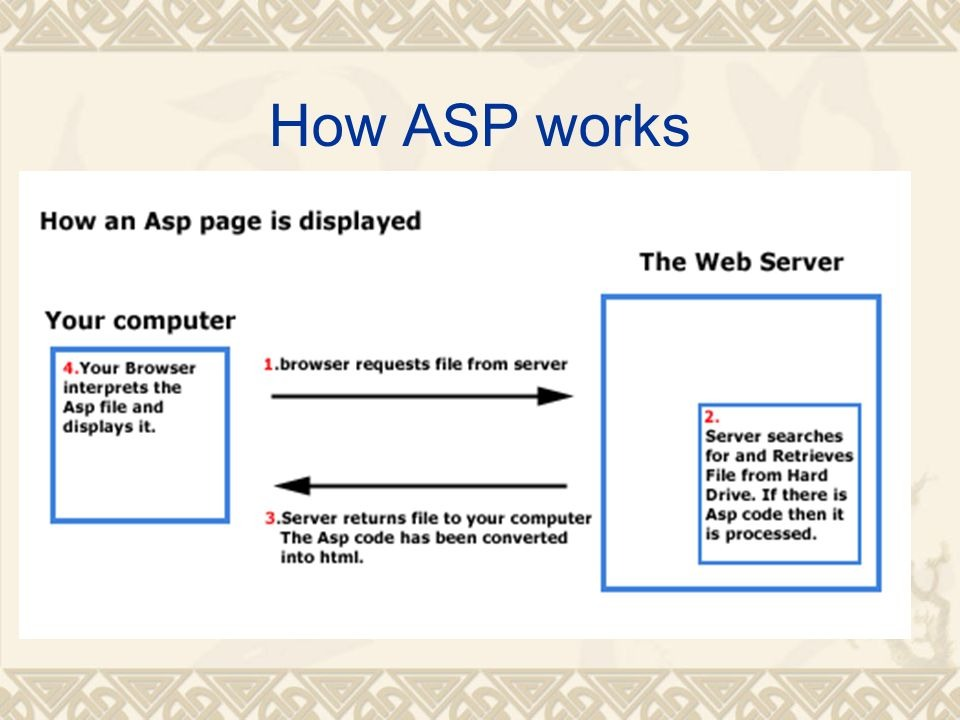
\includegraphics[width=\textwidth]{WhatsApp Image 2023-01-12 at 08.23.16.jpeg}

\subsection{What is session in ASP?}
In ASP session is a state that is used to store and retrieve values of a user. It helps to identify requests from the same browser during a time period (session). It is used to store value for the particular time session. By default, ASP session state is enabled for all ASP applications.

\section{Session variable:}
The most important thing about the Session object is that you can store variables in it.

The example below will set the Session variable username to "Donald Duck" and the Session variable age to "50":

\begin{verbatim}
<%
Session("username")="Donald Duck"
Session("age")=50
%>
\end{verbatim}
When the value is stored in a session variable it can be reached from ANY page in the ASP application:

\begin{verbatim}
Welcome <%Response.Write(Session("username"))%>
\end{verbatim}

\subsection{What is session object?}
A Session object stores information about, or change settings for a user session.
Variables stored in a Session object hold information about one single user, and are available to all pages in one application.

\section{IIS}
Internet Information Services, also known as IIS, is a Microsoft web server that runs on the Windows operating system and is used to exchange static and dynamic web content with internet users. IIS can be used to host, deploy, and manage web applications using technologies such as ASP.NET and PHP.

\section{AJAX? How AJAX works?}
AJAX stands for Asynchronous JavaScript and XML. AJAX is a new technique for creating better, faster, and more interactive web applications with the help of XML, HTML, CSS, and Java Script.

\begin{itemize}
  \item Ajax uses XHTML for content, CSS for presentation, along with Document Object Model and JavaScript for dynamic content display.
  \item Conventional web applications transmit information to and from the sever using synchronous requests. It means you fill out a form, hit submit, and get directed to a new page with new information from the server.
  \item With AJAX, when you hit submit, JavaScript will make a request to the server, interpret the results, and update the current screen. In the purest sense, the user would never know that anything was even transmitted to the server.
  \item XML is commonly used as the format for receiving server data, although any format, including plain text, can be used.
  \item AJAX is a web browser technology independent of web server software.
\end{itemize}

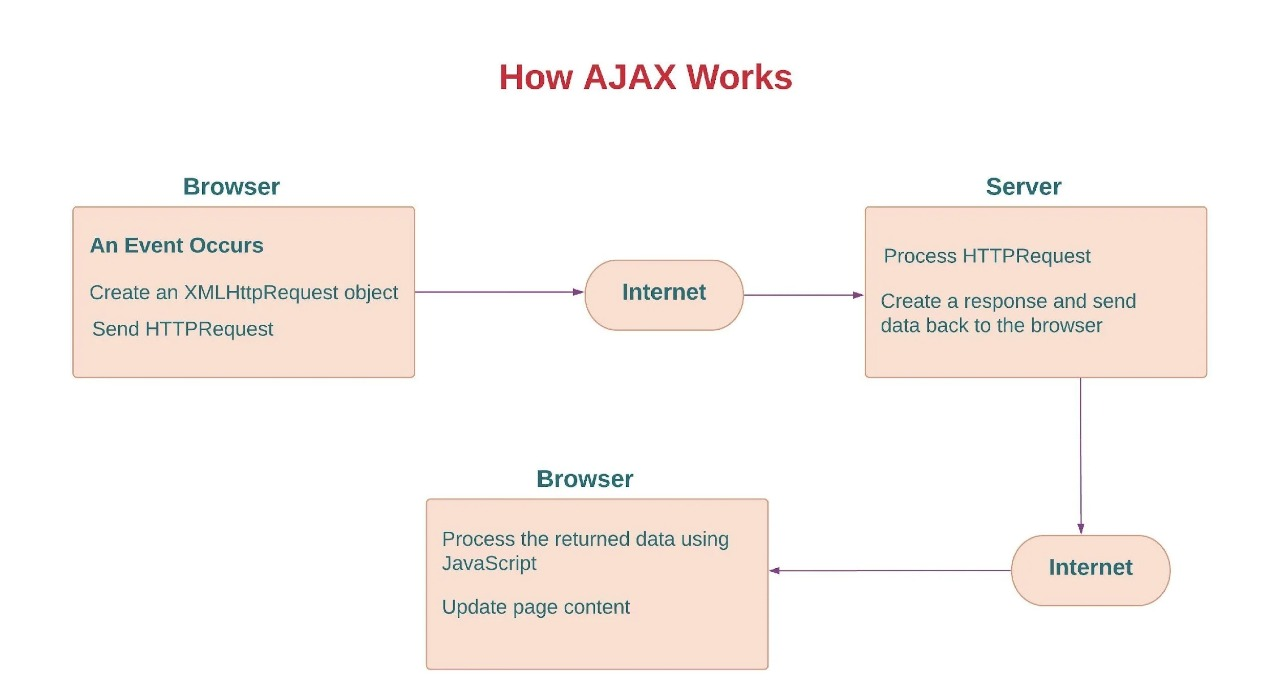
\includegraphics[width=\textwidth]{WhatsApp Image 2023-01-12 at 08.55.03.jpeg}

\subsection{Advantages of AJAX.}
\begin{enumerate}
  \item Reduce server traffic and increase speed: The first and foremost advantage of Ajax is its ability to improve the performance and usability of web applications.
  \item Enable asynchronous calls: Ajax benefits web developers in how its framework can be used for lazy loading.
  \item XMLHttpRequest: XMLHttpRequest is a request type widely used for sending a request to Ajax pages.
  \item Reduce bandwidth usage: One more advantage of Ajax comes from the bandwidth usage.
  \item Form Validation: In contrast to traditional form submission, where client-side validations occur after submission, the AJAX method enables precise and immediate form validation.
\end{enumerate}

\subsection{what is vbscript in ASP?}
VBScript is the simplest language for writing ASP pages. All the code samples in the Creating ASP Pages section are written in VBScript except for samples that are duplicated in JScript for comparison.

\section{What is ActiveX control in asp?}
ActiveX controls are component program objects that Microsoft developed to enable applications to perform specific functions, such as displaying a calendar or playing a video. An ActiveX control is a small program that other applications can reuse to enable the same functionality, without the extra development work.

\section{What is ActiveX control/component used for?}
ActiveX controls are small building blocks that create applications that work over the Internet through Web browsers. Examples include customized applications for collecting data, viewing certain kinds of files, and displaying animation. Common uses of ActiveX controls are command buttons, list boxes, and dialog boxes.

\end{document}
